\documentclass[12pt]{report}
\usepackage{amsmath}
\usepackage{amssymb}
\usepackage{graphicx}
\usepackage{tikz}

\newcommand{\cosec}{\text{ cosec}}
\newcommand{\ubt}[1]{\textbf{\underline{#1}}}
\newcommand{\sps}{\\[0.2cm]}
\newcommand{\spn}[1]{\\[#1cm]}
\newcommand{\refn}[1]{\textbf{(\ref{#1})}}
\newcommand{\refx}[1]{\refn{eq:#1}}
\newcommand{\bt}[1]{\textbf{#1}}
\newcommand{\sprime}{'}
\newcommand{\dprime}{''}
\newcommand{\tprime}{'''}
\newcommand{\dsp}{\displaystyle}
\newcommand{\NI}{\noindent}

\newcommand{\example}[1]{\section*{\ubt{Example #1}}{~}\spn{-1}}
\newcommand{\examples}{\section*{\ubt{Examples}}{~}\spn{-1}}
\newcommand{\solution}{\subsubsection{\ubt{Solution}}{~}\spn{-2}}
\newcommand{\eg}{\section*{\ubt{Example}}{~}\spn{-1}}
\newcommand{\exercise}[1]{\section*{\ubt{Exercise #1}}{~}\spn{-1}}

\renewcommand{\labelenumi}{\arabic{enumi})}
\renewcommand{\labelenumii}{\alph{enumii})}

\renewcommand{\baselinestretch}{1.5}
\renewcommand{\contentsname}{Table of Contents}

\setlength{\parindent}{1em}


\begin{document}
	
	%%%%%%%%%%%%%%%%%%%FRONT COVER%%%%%%%%%%%%%%%%%%%
	\clearpage
	\thispagestyle{empty}
	\addcontentsline{toc}{chapter}{Title Page}
	\begin{center}
		\LARGE \bt{NUMERICAL INTEGRATION USING SIMPSON AND CORRECTED TRAPEZOIDAL}
	\end{center}

	\hspace{7cm}
	
	\begin{center}
		\textbf{\textit{BY}}
	\end{center}
	
	\hspace{5cm}
	
	\begin{center}
		\Large \textbf{Nissi, Wisdom Jerry
			\\
			17/56EB068}
	\end{center}
	
	\hspace{9cm}
	
	\begin{center}
		A PROJECT SUBMITTED TO THE DEPARTMENT OF MATHEMATICS, FACULTY OF PHYSICAL SCIENCES, UNIVERSITY OF ILORIN, ILORIN, KWARA STATE, NIGERIA.
	\end{center}

	\hspace{8cm} \\
	
	\begin{center}
		IN PARTIAL FULFILLMENT OF REQUIREMENTS FOR THE AWARD OF BACHELOR OF SCIENCE \textit{(B.Sc.)} DEGREE IN MATHEMATICS.
	\end{center}
	\hspace{5cm}
	\\ \\ \\
	\begin{center}
		\textbf{FEBRUARY, 2022}
	\end{center}

	\newpage
	\pagenumbering{roman}
	\addcontentsline{toc}{chapter}{\numberline{}Certification}
	\section*{\begin{center}\textbf{\Large Certification}   \end{center}}
	This is to certify that this project was carried out by \textbf{Nissi, Wisdom Jerry} of Matriculation Number  17/56EB068, for the award of Bachelor of Science B.Sc (Hons) degree in the Department of Mathematics, Faculty of Physical sciences, University of Ilorin, Ilorin, Nigeria.
	\\
	\\
	................................... \qquad \qquad\qquad\qquad\qquad\qquad...................... \\
	Prof. M.O. Ibrahim   \hspace{5.5cm} Date\\
	(SUPERVISOR)\\
	\\
	\\
	\\
	...................................... \qquad\qquad\qquad\qquad\qquad\qquad ......................\\
	Prof. K. Rauf    \hspace{6.8cm}    Date\\
	(HEAD OF DEPARTMENT)\\
	\\
	\\
	\\
	..................................... \qquad\qquad\qquad\qquad\qquad\qquad .......................\\
	external  \qquad\qquad\qquad\qquad\qquad\qquad \qquad        Date\\
	(EXTERNAL EXAMINER)
	
	\newpage
	%%ACKNOLEDGEMENT%%
	\section*{\begin{center}\textbf{\Large Acknowledgments}\end{center}}
	\addcontentsline{toc}{chapter}{\numberline{}Acknowledgments} 					
	All thanks to God the Almighty, the one who is and will forever be, the one and only true God, for all He was done for me throughout the course of my academic journey in the University of Ilorin. May the name be praised forever.\\



	\newpage
	%%ABSTRACT%%
	\section*{\begin{center}\textbf{\Large ABSTRACT}\end{center}}
	\addcontentsline{toc}{chapter}{ABSTRACT}
	This project work is concerned with 


	\newpage
	
	%%%%%%%%%%%%%%%%%%%TABLE OF CONTENTS%%%%%%%%%%%%%%%%%%%
	\addcontentsline{toc}{chapter}{Table of Contents}
	\tableofcontents
	
	\newpage
	\pagenumbering{arabic}
	
	%%%%%%%%%%%%%%%%%%%CHAPTER ONE%%%%%%%%%%%%%%%%%%%
	\chapter{GENERAL INTRODUCTION}
	
	\section{Functions}
	A function is a relationship between one variable (the dependent variable) and another variable (the independent variable) or a unique association between members of one set and members of another set. A function from $A$ to $B$ is an object $f$ in which each $a\in A$ is associated with a unique object $f(a) \in B$.\sps
	%
	A function is thus a many-to-one (or in some cases, one-to-one) relationship. The domain of a function is the set $A$ of values at which it is defined. While the function's range is the set of values $f(a)\subset B$ that it can produce. The set $B$ is then referred to as co-domain of $f$. \sps
	%
	Peter Dirichelt, a German mathematician, was the first to give the modern definition of  function in 1837. \textit{``If a variable $y$ is so related to a variable $x$ that whenever a numerical value is assigned to $x$, there is a rule according to which a unique value of $y$ is determined, then $y$ is said to be a function of the independent variable $x$"}.\sps
	%
	The relationship is commonly represented as
	\begin{eqnarray*}
		y=f(x)
	\end{eqnarray*}
	other abbreviated symbols, such as $g(x)$ and $p(x)$ are frequently used to represent functions of the independent variable $x$, particularly when the nature of the function is unknown or unspecified.
	
	\section{Examples of Functions}
	\subsection{Bijective Functions}
	A bijective function is one that is both one-to-one(injective) and onto(surjective).
	
	\begin{figure}[h!]
		\centering
		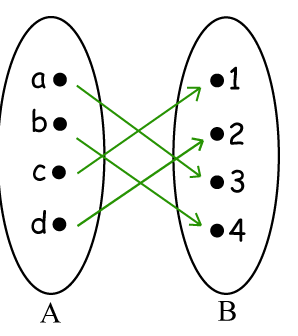
\includegraphics[width=0.3\linewidth]{bijective}
	\end{figure}
	
	\subsection{Composite Functions}
	Let $f$ be a function from set $A$ to set $B$ and let $g$ be a function from set $B$ to set $C$. The composite function of functions $g$ and $f$ denoted as $g \circ f$ is defined by
	\begin{eqnarray*}
		(g\circ f)(x) = g(f(x))
	\end{eqnarray*}
	\begin{figure}[h!]
		\centering
		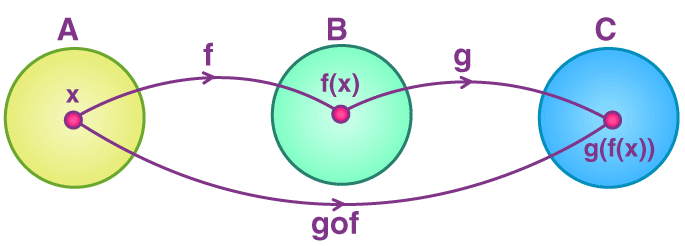
\includegraphics[width=0.5\linewidth]{composite}
	\end{figure}
	
	\subsection{Injective Functions}
	A function $f$ is said to be one-to-one or injective if and only if $f(x) = f(y)$ implies $x=y$ for all $x,y$ in the domain of $f$. A function is said to be injective if it is one-to-one
	\begin{figure}[h!]
		\centering
		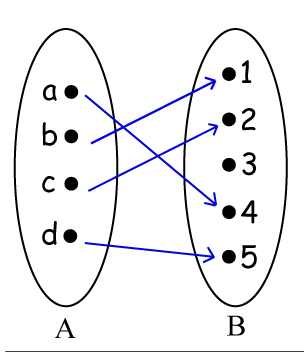
\includegraphics[width=0.3\linewidth]{injective}
	\end{figure}
	
	\subsection{Inverse Functions}
	Let $f$ be a bijective from $A$ to $B$. The inverse function of $f$ is the function that assigned to an element b from $B$. Inverse function of $f$ is denoted by $f^{-1}$. Hence $f^{-1}(b) = a$. When $f(a)=b$. If the inverse function of $f$ exists, $f$ is called invertible.
		\begin{figure}[h!]
		\centering
		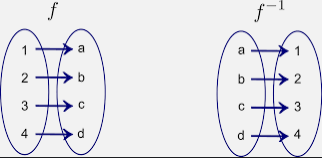
\includegraphics[width=0.35\linewidth]{inverse}
	\end{figure}
	
	
	\subsection{Surjective Functions}
	A function $f$ from $A$ is called onto, or surjective if and only if for every $b\in B$ there is an element $a\in A$ such that $f(a)=b$. All co-domain elements are covered.
	\begin{figure}[h!]
		\centering
		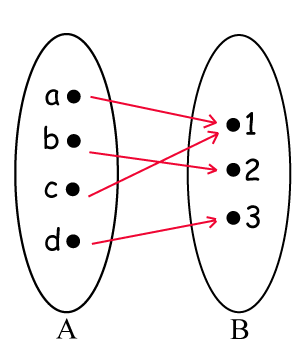
\includegraphics[width=0.3\linewidth]{surjective}
	\end{figure}
	
	
	\section{Integration}
	Integration is the reverse of differentiation. It is a technique for determining a function $g(x)$ whose derivative $g(x)$ is equal to a given function $f(x)$ usually referred to as the indefinite integral sign ``$\int$" as in $\int f(x)$ usually referred to  ss the indefinite integral of the function. The definite integral is written as 
	\begin{eqnarray*}
		\int_a^b f(x) dx
	\end{eqnarray*}
	with $a$ and $b$ called the limits of integration. Some derivatives can be calculated by merely recalling which function has a given derivative. But the techniques of integration mostly involve classifying the function according to which types of manipulations will change the function into a form the anti-derivative of which can be more easily recognized. One useful aid for integration is the theorem known as integration by parts. In symbols, the rule is 
	\begin{eqnarray*}
		\int u dv = uv - \int v du
	\end{eqnarray*}
	That is, if a function is the product of two other function $u$ and one that can be recognized as the derivative of some functions $v$.
	
	\begin{enumerate}
		\item Power Rule: 
			\begin{eqnarray*}
				\int x^n dx = \frac{x^{n+1}}{n+1} + C
			\end{eqnarray*}
		
		\item Exponential Rule:
			\begin{eqnarray*}
				\int e^{kx}dx = \frac{1}{k}e^{kx}+ C
			\end{eqnarray*}
		
		\item Logarithm Rule:
			\begin{eqnarray*}
				\int\frac{1}{x}dx = \ln x + C
			\end{eqnarray*}
	\end{enumerate}
	
	\examples{~}\\[-1.9cm]
	\begin{enumerate}
		\item 
			Find
			\begin{eqnarray*}
				\int x^2\ln x dx
			\end{eqnarray*}
			\solution
			Using integration by parts
			\begin{gather*}
				u=\ln x, ~~\frac{du}{dx} = \frac{1}{x}\sps
				dv = x^2,~~ v = \frac{x^3}{3}
			\end{gather*}
			\begin{eqnarray*}
				\Rightarrow \int u dv &=& uv - \int vdu\sps
				\Rightarrow \int x^2\ln x dx &=& 	\ln\left(\frac{x^3}{3}\right) - \int\frac{x^3}{3}\cdot \frac{1}{x}dx\sps
				\Rightarrow && \frac{x^3}{3}\ln x - \frac{1}{3}\int x^2 	dx\sps
				\Rightarrow && \frac{x^3}{3}\ln x - 	\frac{1}{3}\left(\frac{x^3}{3}\right) + C \sps
				\Rightarrow && \frac{x^3}{3}\left(\ln x - 	\frac{1}{3}\right) + C
			\end{eqnarray*}
	
		\item
			Find
			\begin{eqnarray*}
				\int (2x^5 + 8x^3 - 3x^2 + 5)dx
			\end{eqnarray*}
			\solution{~}\\[-1.7cm]
			\begin{eqnarray*}
				&=& 2\int x^5 dx + 8\int x^3dx - 3\int x^2 dx + 5\int dx\sps
				&=& 2\left(\frac{x^6}{6}\right)+ 8\left(\frac{x^4}{4}\right) - 3\left(\frac{x^3}{3}\right) + 5(x) + C\sps
				&=& \frac{2x^6}{6} + \frac{8x^4}{4} - \frac{3x^3}{3} + 5x + C\sps
				&=&\frac{x^6}{3} + 2x^4 - x^3 + 5x + C
			\end{eqnarray*}
	\end{enumerate}


	\section{Various way of Integrating}
	\subsection{Integrating by Substitution}
	\eg
	Find 
	\begin{equation}
		\int (2x + 7)^{1/2}dx\tag{1}\label{tag:sub:1}
	\end{equation}
	\solution
	Let $\dsp u=2x + 7 \Rightarrow \frac{du}{dx} = 2 \Rightarrow dx = \frac{du}{2}$ \sps
	By substituting in \refn{tag:sub:1}
	\begin{eqnarray*}
		\int u^{1/2} \cdot \frac{du}{2} &=& \frac{\frac{1}{2} u^{1/2 + 1}}{\frac{1}{2}+1} + C\sps
		&=& \frac{\frac{1}{2}u^{3/2}}{\frac{3}{2}} + C \sps
		&=& \frac{1}{3}u^{3/2} + C\sps
		&=& \frac{1}{3}\left(2x + 7\right)^{3/2} + C
	\end{eqnarray*}
	
	
	\subsection{Integration in Exponential Form}
	\eg
	Find
	\begin{eqnarray*}
		\int 3x^{4x}dx
	\end{eqnarray*}
	\solution
	Let $u = 4x$, then $du = 4dx$
	\begin{eqnarray*}
		\Rightarrow \int 3e^{4x}dx &=& \int 3e^{u} \cdot \frac{du}{4}\sps
		&=& \frac{3}{4}\int e^u du\sps
		&=& \frac{3}{4}e^u + k\sps
		&=& \frac{3}{4}e^{4x} + k
	\end{eqnarray*}
	
	\subsection{Integration by Trigonometric Substitution}
	\eg
	Find
	\begin{eqnarray*}
		\int\frac{dx}{\sqrt{x^2 + 2x}}
	\end{eqnarray*}
	\solution
	Let assume $x^2 + 2x = (x+1)^2 - 1$\\
	Put $u = x+1, \Rightarrow du = dx$.\\
	Thus
	\begin{eqnarray*}
		\int\frac{dx}{\sqrt{x^2 + 2x}} = \int \frac{du}{\sqrt{u^2 - 1}}
	\end{eqnarray*}	
	Let $u = \sec\theta$ and $du = \sec\theta\tan\theta d \theta$\\
	also,
	\begin{eqnarray*}
		\sqrt{u^2 - 1} = \sqrt{\sec^2\theta - 1} = \sqrt{\tan^2\theta} = \tan\theta
	\end{eqnarray*}
	So we have,
	\begin{eqnarray*}
			\int\frac{dx}{\sqrt{x^2 + 2x}} &=& \int\frac{du}{\sqrt{u^2 - 1}} = \int\frac{\sec\theta\tan\theta d\theta}{\tan \theta}\sps
			&=& \int \sec\theta d\theta\sps
			&=& \ln(\sec\theta) + \ln(\theta) + K\sps
			&=& \ln(\sec\theta + \tan\theta) + K
	\end{eqnarray*}
	Inserting back, we have
	\begin{gather*}
		\sec\theta \Rightarrow u = x + 1\sps
		\tan\theta = \sqrt{u^2 - 1}\sps
		\Rightarrow \ln(x+1 + \sqrt{x^2 + 2x}) + K
	\end{gather*}
	
	\subsection{Integration by Parts}
	We have $\dsp \int udv = uv - \int v du$
	\eg
	Find
	\begin{eqnarray*}
		\int x \sin 2x dx
	\end{eqnarray*}
	\solution
	Let
	\begin{gather*}
		u=x, dv = \sin 2x\sps
		du =dx, v = -\frac{\cos 2x}{2}
	\end{gather*}
	Substituting into the integration by parts formula
	\begin{eqnarray*}
		\int x\sin 2x dx &=& x\left[-\frac{\cos 2x}{2}\right] - \int -\frac{\cos 2x}{2}dx\sps
		&=& - \frac{x\cos 2x}{2} + \frac{1}{2}\int\cos 2x dx\sps
		&=& -\frac{x\cos2x}{2} + \frac{1}{2}\left[\frac{\sin2x}{2}\right] + K\sps
		&=& -\frac{x\cos 2x}{2} + \frac{\sin2x}{4} + K
	\end{eqnarray*}
	
	\subsection{Integration by Partial Fractions}
	\eg
	Find
	\begin{eqnarray*}
		\int \frac{4}{x^2-4}dx
	\end{eqnarray*}
	\solution
	\begin{eqnarray*}
		\int \frac{4}{x^2-4}dx = \int\frac{4}{(x-2)(x+2)}dx
	\end{eqnarray*}
	By partial fraction
	\begin{eqnarray*}
		\frac{4}{(x-2)(x+2)} = \frac{A}{(x-2)} + \frac{B}{(x+2)}
	\end{eqnarray*}
	multiply both side by $(x-2)(x+2)$
	\begin{gather*}
		4 = A(x+2) + B(x-2)\sps
		4 = Ax + 2A + Bx - 2B
	\end{gather*}
	Let the coefficient of $x$ be
	\begin{eqnarray*}
		0 &=& A + B\sps
		A &=& - B\sps
		4 &=& 2A - 2B\sps
		4 &=&2(-B) - 2B\sps
		\frac{4}{4} &=& -\frac{4B}{4}, B=-1, A=1
	\end{eqnarray*}
	\begin{eqnarray*}
		\frac{4}{(x-2)(x+2)} = \frac{1}{x-2}+ \frac{-1}{x+2}
	\end{eqnarray*}
	By integrating
	\begin{eqnarray*}
		\int \frac{4}{(x-2)(x+2)} &=& \int \frac{1}{(x-2)}dx - \int\frac{1}{(x+2)}dx\sps
		&=& \ln(x-2) - \ln(x+2) + C\sps
		&=& \ln\left(\frac{x-2}{x+2}\right) + C
	\end{eqnarray*}
	
	
	
	
	
	
	
	
	
%	
%	\section{STATEMENT OF THE PROBLEM}
%
%	
%	\section{AIMS AND OBJECTIVES OF THE STUDY}
%	
%	\section{SIGNIFICANCE OF STUDY}
%
%	
%	\section{SCOPE OF THE STUDY}
%	
	

	
	%%%%%%%%%%%%%%%%%%%CHAPTER TWO%%%%%%%%%%%%%%%%%%%
	\chapter{NUMERICAL INTEGRATION}
	In analysis, numerical integration comprises a broad family of algorithms for calculating the numerical value of a definite integral, and by extension, the term is also sometimes used to describe the numerical solution of differential equations.\sps
	The basic problem in numerical integration is to compute an approximate solution to a definite integral
	\begin{eqnarray}
		\int_a^b f(x) dx
	\end{eqnarray}
	to a given degree of accuracy. If $f(x)$ is a smooth function integrated over a small number of dimensions, and the domain of integration is bounded, there are many methods for approximating the integral to the desired precision.\sps
	The Integrand $f(x)$ may be known only at certain points, such as obtained by sampling some embedded systems and other computer applications may need numerical integration for this reason.\sps
	A formula for the integrand may be known but it may be difficult or impossible to find an anti-derivative that is an elementary function. It may be possible to find an anti-derivative symbolically but it may be easier to compute the anti-derivative that may be the case, if the anti-derivative is given as an infinite series or product or its evaluation requires a special function that is not available.\sps
	Newton-Cotes formula evaluates the function $F$ at a finite number of points between $[a,b]$ and uses this point to build an interpolation between these points typically a linear approximation in most of the cases. Then this value is integrated to get an approximate value of the integral.
	
	\section{Quadrature Rules base on Interpolating Functions}
	A large class of quadrature rules can be derived by constructing interpolating functions that are easy to integrate. Typically these interpolating functions are polynomials. In practice, since polynomials of very high degree tend to oscillate wildly, only polynomials of low degree are used, typically linear and quadratic.\sps
	The simplest method of this type is to let the interpolating function be a constant function (a polynomial of degree zero) that passes through the point $\dsp \left(\frac{a+b}{2}, f\left(\frac{a+b}{2}\right)\right)$. This is call the midpoint rule and 
	\begin{eqnarray}
		\int_a^b f(x) dx \approx  \left(\frac{a+b}{2}, f\bigg(\frac{a+b}{2}\bigg)\right)
	\end{eqnarray}

	\NI The interpolating function may be a straight line(an affine function, i.e a polynomial of degree 1) passing through the points $(a,f(a))$ and $(b,f(b))$. This is called the trapezoidal rule and
	\begin{eqnarray}
		\int_a^b f(x) dx \approx (b-a)\left(\frac{f(a) + f(b)}{2}\right)
	\end{eqnarray}
	
	\subsection{Simpson's Rule}
	In numerical integration, Simpson's rules are several approximations for definite integrals, named after Thomas Simpson (1710 - 1761)
	\begin{figure}[!h]
		\centering
		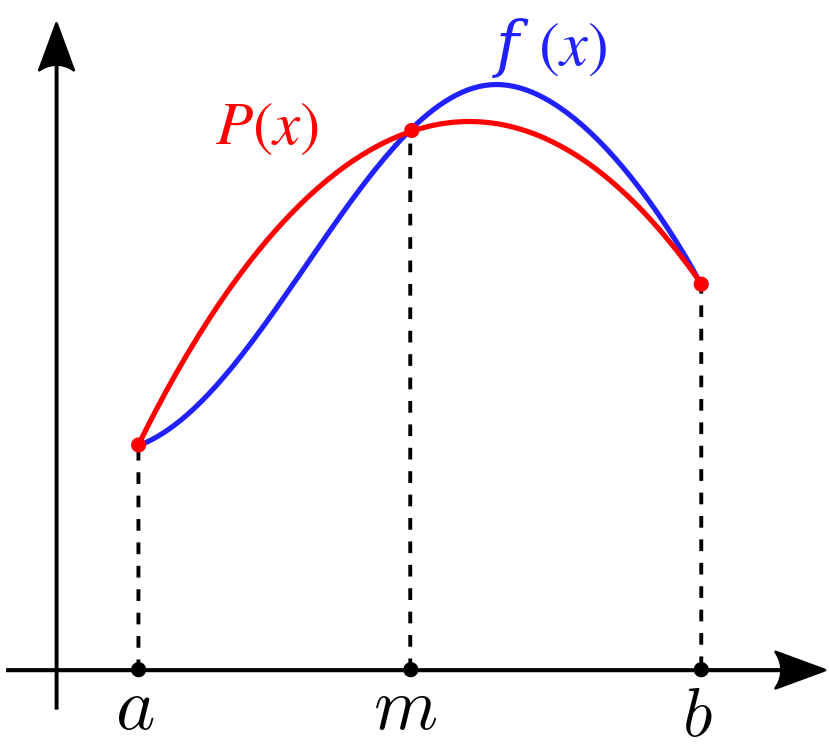
\includegraphics[width=.4\linewidth]{Simpsons_method_illustration}
	\end{figure}
	\NI Simpson's rule can be derived by approximating the integrand $f(x)$ by the quadratic interpolant $p(x)$.\sps
	The most basic of these rules, called Simpson's $1/3$ rule or just Simpson's rule read
	\begin{eqnarray}
		\int_a^b f(x) dx \approx \frac{b-a}{6}\left[f(a)+ 4f\left(\frac{a+b}{2}\right) + f(b) \right]  
	\end{eqnarray}
	for German and some other languages, it is named after Johannes Kepler, who derived it in 1615 after seeing it used for wine barrels(barrel rule, Keplersche Fassregel). The approximate equality in the rule becomes exact if $f$ is a polynomial up to 3rd degree.
	
	\subsubsection{Derivation of Simpson's Rule}
	One derivation replaces the integrand $f(x)$ by the quadratic polynomial (i.e parabola) $p(x)$ that takes the same values as $f(x)$ at the endpoints $a$ and $b$ and the midpoint $\dsp m = \left(\frac{a+b}{2}\right)$. One can use Lagrange polynomial interpolation to find an expression for this polynomial,
	\begin{eqnarray*}
		p(x) = f(a) \frac{(x-m) (x-b)}{(a-m) (a-b)} + f(m) \frac{(x-a)(x-b)}{(m-a) (m-b)} + f(b)\frac{(x-a)(x-m)}{(b-a) (b-m)}
	\end{eqnarray*}	
	Using integration by substitution, one can show that 
	\begin{eqnarray}
		\int_a^b p(x) dx = \frac{b-a}{6}\left[f(a)+ 4f\left(\frac{a+b}{2}\right) + f(b) \right]  \label{eq:2_5}
	\end{eqnarray}
	Introducing the step size $\dsp h = \frac{(b-a)}{2}$, thus \refx{2_5} is also commonly written as
	\begin{eqnarray}
			\int_a^b p(x) dx = \frac{h}{3}\left[f(a)+ 4f\left(\frac{a+b}{2}\right) + f(b) \right]\\\notag
	\end{eqnarray}
	
	\NI Because of the $1/3$ factor, Simpson's rule is also referred to as ``Simpson's $1/3$ rule''
	
	\subsection{Averaging the Midpoint and the Trapezoidal Rules}
	Another derivatives constructs Simpson's rule from two simpler approximations: the midpoint rule
	\begin{eqnarray}
		M = (b-a) f\left(\frac{a+b}{2}\right)
	\end{eqnarray}
	and the trapezoidal rule
	\begin{eqnarray}
		T = \frac{1}{2}(b-a) (f(a) + f(b))
	\end{eqnarray}
	
	\NI The errors in these approximations are 
	\begin{eqnarray*}
		\frac{1}{24}(b-a)^3 f''(a) + O((b-a)^4)
	\end{eqnarray*}
	and 
	\begin{eqnarray*}
		-\frac{1}{12}(b-a)^3 f''(a) + O((b-a)^4)
	\end{eqnarray*}
	respectively, where $O((b-a)^4)$ denotes a term asymptotically proportional to $(b-a)^4$. The two $O((b-a)^4)$ terms are not equal to follows from the above formulas for the errors of the midpoint and trapezoidal rule that the leading error terms vanishes if we take the weighted average
	\begin{eqnarray*}
		\frac{2M + T}{3}
	\end{eqnarray*}
	This weighted average is exactly Simpson's rule.
	
	\subsection{Trapezoidal Rule}
	In mathematics, and more specifically in numerical analysis, the trapezoidal rule (also known as the trapezoidal rule or trapezium rule) is a technique for approximating the definite integral.
	\begin{eqnarray*}
		int_a^b f(x) dx
	\end{eqnarray*}
	The trapezoidal rule works by approximating the region under the graph of the function $f(x)$ as a trapezoidal and calculating its area. It follows that
	\begin{eqnarray*}
		\int_a^b f(x) dx \approx \frac{1}{2}(b-a)\left[f(a)+f(b)\right]
	\end{eqnarray*}

	\section{Error Analysis}
	The error of the composite trapezoidal rule is the difference between the value of the integral and the numerical result:
	\begin{eqnarray*}
		E = \int_a^b f(x) dx  - \frac{b-a}{N}\left[\frac{f(a) + f(b)}{2} + \sum_{k=1}^{N-1} f\left(a + k\frac{b-a}{N}\right) \right] 
	\end{eqnarray*}
	There exists a number $\epsilon$ between $a$ and $b$, such that
	\begin{eqnarray*}
		E = - \frac{(b-a)^3}{2N^2}f''(\epsilon)
	\end{eqnarray*}
	An asymptotic error estimate for $N\to\infty$ is given by 
	\begin{eqnarray*}
		E = - \frac{(b-a)^2}{2N^2}\bigg[ f'(b) - f'(a)\bigg] + O(N^{-3})
	\end{eqnarray*}
	
	%%%%%%%%%%%%%%%%%%%CHAPTER THREE%%%%%%%%%%%%%%%%%%%
	\chapter{SOLVED EXAMPLES}
	%In this chapter, three problems was solved by Closed Newton-Cotes Formulae and the results obtained  were compared with the exact solution.\\
	\section{Solved Examples on Rectangle Rule}
	\subsection{Example 1}
	Using Rectangle rule, solve
	\begin{gather*}
		I = \int_1^3\left(x^3 - 2x^2 + 7x - 5\right)dx
	\end{gather*}
	\subsection*{Solution}
	{~}\\[-2.1cm]
	\begin{eqnarray*}
		f(x) = x^3 - 2x^2 + 7x - 5\sps
		b = 3,~~ a = 1
	\end{eqnarray*}
	{~}\\[-2.1cm]
	\begin{gather*}
		\text{Rectangle rule} = b-af(a)
	\end{gather*}
	{~}\\[-2.1cm]
	\begin{eqnarray*}
		&=&(3-1)(1^3 - 2(1)^2 + 7(1) - 5)\sps
		&=&(2)(1-2+7-5)\sps
		&=&(2)(1)\sps
		&=&2
	\end{eqnarray*}
	
	\subsection{Example 2}
	Using Rectangle rule, solve
	\begin{eqnarray*}
		I = \int_0^1\left(x^3 + 3x + 1\right)dx
	\end{eqnarray*}

	\subsection*{Solution}
	{~}\\[-2.1cm]
	\begin{gather*}
		f(x) = x^3 + 3x + 1\sps
		b=1,~~ a = 0
	\end{gather*}
	{~}\\[-2.1cm]
	\begin{gather*}
		\text{Rectangle rule} = b-af(a)
	\end{gather*}
	{~}\\[-2.1cm]
	\begin{eqnarray*}
		&=&(1-0)(0^3 + 3(0) + 1)\sps
		&=&(1)(1)\sps
		&=&1
	\end{eqnarray*}
	
	\subsection{Example 3}
	Using Rectangle rule, solve
	\begin{eqnarray*}
		I = \int_2^5\left(x^5 + 2x^4 + 3x^2 + 2\right)dx
	\end{eqnarray*}
	
	\subsection*{Solution}
	{~}\\[-2.1cm]
	\begin{gather*}
		f(x) = x^5 + 2x^4 + 3x^2 + 2\sps
		b=5,~~ a = 2
	\end{gather*}
	{~}\\[-2.1cm]
	\begin{gather*}
		\text{Rectangle rule} = b-af(a)
	\end{gather*}
	{~}\\[-2.1cm]
	\begin{eqnarray*}
		&=&(5-2)(2^5 + 2(2)^4 + 3 (2)^2 + 2)\sps
		&=&(3)(32+32+12+2)\sps
		&=&(3)(78)\sps
		&=&234
	\end{eqnarray*}
	
	\section{Solved Examples on Midpoint Rule}
	\subsection{Example 1}
	Using Midpoint rule, solve
	\begin{eqnarray*}
		I = \int_1^3\left(x^3 - 2x^2 + 7x - 5\right)dx
	\end{eqnarray*}
	
	\subsection*{Solution}
	{~}\\[-2.1cm]
	\begin{gather*}
		f(x) = x^3 - 2x^2 + 7x - 5\sps
		b=3,~~ a=1
	\end{gather*}
	{~}\\[-2.1cm]
	\begin{gather*}
		\text{Midpoint rule} = b-af\left(\frac{a+b}{2}\right)
	\end{gather*}
	{~}\\[-2.1cm]
	\begin{eqnarray*}
		&=&(3-1)f\left(\frac{1+3}{2}\right)\sps
		&=&(3-1)f\left(\frac{4}{2}\right)\sps
		&=&(2)f(2)\sps
		&=&(2)(2^3-2(2)^2 + 7(2)-5)\sps
		&=&(2)(9)\sps
		&=&18
	\end{eqnarray*}
	
	\subsection{Example 2}
	Using Midpoint rule, solve
	\begin{eqnarray*}
		I = \int_0^1\left(x^3 + 3x + 1\right)dx
	\end{eqnarray*}
	
	\subsection*{Solution}
	{~}\\[-2.1cm]
	\begin{gather*}
		f(x) = x^3 + 3x + 1\sps
		b=1, a=0
	\end{gather*}
	{~}\\[-2.1cm]
	\begin{gather*}
		\text{Midpoint rule} = b-af\left(\frac{a+b}{2}\right)
	\end{gather*}
	{~}\\[-2.1cm]
	\begin{eqnarray*}
		&=&(1-0)f\left(\frac{0+1}{2}\right)\sps
		&=&(1)f\left(\frac{1}{2}\right)\sps
		&=&(1)\left(\left(\frac{1}{2}\right)^2 + 3\left(\frac{1}{2}\right) + 1\right)\sps
		&=&(1)\left(\frac{1}{8} + \frac{3}{2} + 1\right)\sps
		&=&\frac{21}{8}
	\end{eqnarray*}
	
	\subsection{Example 3}
	Using Midpoint rule, solve
	\begin{eqnarray*}
		I = \int_2^5\left(x^5 + 2x^4 + 3x^2 + 2\right)dx
	\end{eqnarray*}
	
	\subsection*{Solution}
	{~}\\[-2.1cm]
	\begin{gather*}
		f(x) = x^5 + 2x^4 + 3x^2 + 2\sps
		b=5, a=2
	\end{gather*}
	{~}\\[-2.1cm]
	\begin{gather*}
		\text{Midpoint rule} = b-af\left(\frac{a+b}{2}\right)
	\end{gather*}
	{~}\\[-2.1cm]
	\begin{eqnarray*}
		&=&(5-2)f\left(\frac{2+5}{2}\right)\sps
		&=&(3)f\left(\frac{7}{2}\right)\sps
		&=&(3)\left(\left(\frac{7}{2}\right)^5 + 2\left(\frac{7}{2} \right)^4+ 3\left(\frac{7}{2}\right)^2 + 2\right)\sps
		&=&(3)\left(\frac{27651}{32}\right)\sps
		&\implies& \frac{82953}{32}
	\end{eqnarray*}


	\section{Solved Examples on Trapezoidal Rule}
	\subsection{Example 1}
	Using trapezoidal rule, solve
	\begin{eqnarray*}
		I = \int_1^3\left(x^3 - 2x^2 + 7x - 5\right)dx
	\end{eqnarray*}
	
	\subsection*{Solution}
	{~}\\[-2.1cm]
	\begin{gather*}
		f(x) = x^3 - 2x^2 + 7x - 5\sps
		b=3,~~ a=1
	\end{gather*}
	{~}\\[-2.1cm]
	\begin{gather*}
		\text{Trapezoidal rule} = \frac{1}{2}(b-a)[f(a) + f(b)]
	\end{gather*}
	{~}\\[-2.1cm]
	\begin{eqnarray*}
		&\implies&\frac{1}{2}(3-1)\left[(1^3-2(1)^2 + 7(1)-5) + (3^3 - 2(3)^2) + 7(3) - 5)\right] \sps
		&\implies&\frac{1}{2}(2)\left[(1-2+7-5) + (27-18 + 21-5)\right]\sps
		&\implies&[1+25]\sps
		&\implies& 26
	\end{eqnarray*}
	
	\subsection{Example 2}
	Using trapezoidal rule, solve
	\begin{eqnarray*}
		I = \int_0^1\left(x^3 + 3x + 1\right)dx
	\end{eqnarray*}
	
	\subsection*{Solution}
	{~}\\[-2.1cm]
	\begin{gather*}
		f(x) = x^3 + 3x + 1\sps
		b=1,~~ a=0
	\end{gather*}
	{~}\\[-2.1cm]
	\begin{gather*}
		\text{Trapezoidal rule} = \frac{1}{2}(b-a)[f(a) + f(b)]
	\end{gather*}
	{~}\\[-2.1cm]
	\begin{eqnarray*}
		&\implies&\frac{1}{2}(1-0)[(0^3 + 3(0) + 1) + (1^3 + 3(1) + 1)]\sps
		&\implies& \frac{1}{2}(1)[1+5]\sps
		&\implies&\frac{1}{2}[6]\sps
		&\implies& 3
	\end{eqnarray*}
	
	\subsection{Example 3}
	Using trapezoidal rule, solve
	\begin{eqnarray*}
		I = \int_2^5\left(x^5 + 2x^4 + 3x^2 + 2\right)dx
	\end{eqnarray*}
	
	\subsection*{Solution}
	{~}\\[-2.1cm]
	\begin{gather*}
		f(x) = x^5 + 2x^4 + 3x^2 + 2\sps
		b=2,~~ a=5
	\end{gather*}
	{~}\\[-2.1cm]
	\begin{gather*}
		\text{Trapezoidal rule} = \frac{1}{2}(b-a)[f(a) + f(b)]
	\end{gather*}
	{~}\\[-2.1cm]
	\begin{eqnarray*}
		&\implies&\frac{1}{2}(5-2)[(2^5 + 2(2)^4 + 3(2)^2 + 2) + (5^5 + 2(5)^4+3(5)^2 + 2)]\sps
		&\implies& \frac{1}{2}(3)[(32+32+12+2) + (3125+1250+75+2)]\sps
		&\implies& \frac{3}{2}[78+445]\sps
		&\implies& \frac{3}{2}[4530]\sps
		&\implies& \frac{13590}{2}\sps
		&\implies& 6795
	\end{eqnarray*}
	
	\section{Solved Examples on Simpson's Rule}
	\subsection{Example 1}
	Using Simpson's rule, solve
	\begin{eqnarray*}
		I = \int_1^3\left(x^3 - 2x^2 + 7x - 5\right)dx
	\end{eqnarray*}
	
	\subsection*{Solution}
	{~}\\[-2.1cm]
	\begin{gather*}
		f(x) = x^3 - 2x^2 + 7x - 5\sps
		b=3,~~ a=1
	\end{gather*}
	{~}\\[-2.1cm]
	\begin{gather*}
		\text{Simpson's rule} = \frac{b-a}{6}\left[f(a)+ 4f\left(\frac{a+b}{2}\right) + f(b)\right]
	\end{gather*}
	{~}\\[-1.5cm]
	\begin{eqnarray*}
		&\implies&\frac{3-1}{6}\left[(1^3 -2(1)^2 + 7(1)-5)+ 4f\left(\frac{1+3}{2}\right)+(3^3 - 2(3)^2) + 7(3)-5\right]\sps
		&\implies& \frac{2}{6}\left[(1-2+7-5) + 4(2^3 - 2(2)^2 + 7(2)-5) + (27-18+21-5)\right]\sps
		&\implies& \frac{1}{3}[1+36+25]\sps
		&\implies& \frac{62}{3}
	\end{eqnarray*}
	
	
	\subsection{Example 2}
	Using Simpson's rule, solve
	\begin{eqnarray*}
		I = \int_0^1\left(x^3 +3x + 1\right)dx
	\end{eqnarray*}
	
	\subsection*{Solution}
	{~}\\[-2.1cm]
	\begin{gather*}
		f(x) = x^3 +3x + 1\sps
		b=1,~~ a=0
	\end{gather*}
	{~}\\[-2.1cm]
	\begin{gather*}
		\text{Simpson's rule} = \frac{b-a}{6}\left[f(a)+ 4f\left(\frac{a+b}{2}\right) + f(b)\right]
	\end{gather*}
	{~}\\[-2.1cm]
	\begin{eqnarray*}
		&\implies&\frac{1-0}{6}\left[(0^3 + 3(0) + 1) + 4f\left(\frac{0+1}{2}\right)+ (1^3 + 3(1) + 1)\right]\sps
		&\implies& \frac{1}{6}\left[1+4f\left(\frac{1}{2}\right)+5\right]\sps
		&\implies&\frac{1}{6}\left[1+4\left(\frac{1}{8}+\frac{3}{2}+1\right)+5\right]\sps
		&\implies&\frac{1}{6}\left[\frac{33}{2}\right]\sps
		&\implies& \frac{11}{4}
	\end{eqnarray*}
	
	
	\subsection{Example 3}
	Using Simpson's rule, solve
	\begin{eqnarray*}
		I = \int_2^5\left(x^5 + 2x^4 + 3x^2 + 2\right)dx
	\end{eqnarray*}
	
	\subsection*{Solution}
	{~}\\[-1.9cm]
	\begin{gather*}
		f(x) = x^5 + 2x^4 + 3x^2 + 2\\[-0.2cm]
		b=5,~~ a=2
	\end{gather*}
	{~}\\[-1.9cm]
	\begin{gather*}
		\text{Simpson's rule} = \frac{b-a}{6}\left[f(a)+ 4f\left(\frac{a+b}{2}\right) + f(b)\right]
	\end{gather*}
	{~}\\[-1.5cm]
	\begin{eqnarray*}
		&\implies& \frac{5-2}{6}\left[(2^5 + 2(2)^4 + 3(2)^2 + 2) + 4f\left(\frac{7}{2}\right) + (3125+1250+75+2)\right]\sps
		&\implies&\frac{3}{6}\left[78+\frac{27651}{32}+ 4452\right]\sps
		&\implies& \frac{1}{2}\left[\frac{172611}{32}\right]\sps
		&\implies& \frac{172611}{64}
	\end{eqnarray*}

	
	
	\section{Solved Examples on Corrected Trapezoidal Rule}
	\subsection{Example 1}
	Using corrected trapezoidal rule, solve
	\begin{eqnarray*}
		I = \int_1^3\left(x^3 - 2x^2 + 7x - 5\right)dx
	\end{eqnarray*}
	
	\subsection*{Solution}
	{~}\\[-2.1cm]
	\begin{gather*}
		f(x) = x^3 - 2x^2 + 7x - 5\sps
		f\sprime(x) = 3x^2 - 4x + 7\sps
		b=3,~~ a=1
	\end{gather*}
	{~}\\[-2.1cm]
	\begin{gather*}
		\text{Corrected trapezoidal rule} = \frac{b-a}{2}\Big[f(a) + f(b)\Big] + \frac{(b-a)^2}{12}\Big[f\sprime(a)-f\sprime(b)\Big]
	\end{gather*}
	{~}\\[-1.5cm]
	\begin{eqnarray*}
		&\implies&\frac{3-1}{2}\left[(1^2-2(1)^2 + 7(1) - 5) + (3^3 - 2(3)^2 + 7(3) - 5)\right]\sps
		&& +\frac{(3-1)^2}{12}\left[(3(1)^2 - 4(1) + 7) - (3(3)^2 - 4(3) + 7)\right]\spn{0.4}
		&\implies& 1\Big[(1-2+7-5) + (27-18+21-5)\Big] + \frac{4}{12}\Big[(3-4+7)- (27-12+7)\Big]\spn{0.4}
		&\implies&\Big[1+25\Big]+ \frac{1}{3}\Big[6-22\Big]\spn{0.4}
		&\implies& 26 + \left(-\frac{16}{3}\right)\spn{0.4}
	\end{eqnarray*}
	\begin{eqnarray*}
		&\implies& 26 - \frac{16}{3}\hspace{10cm}\spn{0.4}
		&\implies& \frac{62}{3}
	\end{eqnarray*}
	
	
		\subsection{Example 2}
	Using corrected trapezoidal rule, solve
	\begin{eqnarray*}
		I = \int_0^1\left(x^3 +3x + 1\right)dx
	\end{eqnarray*}
	
	\subsection*{Solution}
	{~}\\[-2.1cm]
	\begin{gather*}
		f(x) = x^3 +3x + 1\sps
		f\sprime(x) = 3x^2 + 3\sps
		b=1,~~ a=0
	\end{gather*}
	{~}\\[-2.1cm]
	\begin{gather*}
		\text{Corrected trapezoidal rule} = \frac{b-a}{2}\Big[f(a) + f(b)\Big] + \frac{(b-a)^2}{12}\Big[f\sprime(a)-f\sprime(b)\Big]
	\end{gather*}
	{~}\\[-1.5cm]
	\begin{eqnarray*}
		&\implies&\frac{1-0}{2}\left[ (0^3 + 3(0) + 1) + (1^3 + 3(1) + 1) \right]\sps
		&& +\frac{(1-0)^2}{12}\left[ (3(0)^2 + 3) - (3(1)^2 + 3) \right]\spn{0.4}
		&\implies&\frac{1}{2}\left[(1) + (5)\right]+ \frac{1}{2}\left[3-6\right]\spn{0.4}
		&\implies&\frac{1}{2}\left[6\right]+ \frac{1}{12}\left[-3\right]\spn{0.4}
		&\implies& 3 - \frac{3}{12}\spn{0.4}
		&\implies&\frac{11}{4}
	\end{eqnarray*}
	
	
	
	\subsection{Example 3}
	Using corrected trapezoidal rule, solve
	\begin{eqnarray*}
		I = \int_2^5\left(x^5 + 2x^4 + 3x^2 + 2\right)dx
	\end{eqnarray*}
	
	\subsection*{Solution}
	{~}\\[-2.1cm]
	\begin{gather*}
		f(x) = x^5 + 2x^4 + 3x^2 + 2\sps
		f\sprime(x) = 5x^4 + 8x^3 + 6x \sps
		b=5,~~ a=2
	\end{gather*}
	{~}\\[-2.1cm]
	\begin{gather*}
		\text{Corrected trapezoidal rule} = \frac{b-a}{2}\Big[f(a) + f(b)\Big] + \frac{(b-a)^2}{12}\Big[f\sprime(a)-f\sprime(b)\Big]
	\end{gather*}
	{~}\\[-1.5cm]
	\begin{eqnarray*}
		&\implies&\frac{5-2}{2}\left[ (2^5 + 2(2)^4 + 3(2)^2 + 2) + (5^5 + 2(5)^4 + 3(5)^2 + 2) \right]\sps
		&& +\frac{(5-2)^2}{12}\left[ (5(2)^4 + 8(2)^3 + 6(2)) + (5(5)^4 + 8(5)^3 + 6(5))  \right]\spn{0.4}
		&\implies& \frac{3}{2}[(32+32+12+2) + (3125+1250+75+2)] \sps
		&& +\frac{3}{4}\left[ (80+64412) - (3125+1000+30) \right]   \spn{0.4}
		&\implies&  \frac{3}{2}[78+4452] + \frac{3}{4}[156 - 4155] \spn{0.4}
		&\implies& \frac{13590}{2} + \left(\frac{-11997}{4}\right)\spn{0.4}
		&\implies&\frac{13590}{2} - \frac{11997}{4}\spn{0.4}
		&\implies& \frac{15183}{4} 
	\end{eqnarray*}
	
	
	%%%%%%%%%%%%%%%%%%%CHAPTER FOUR%%%%%%%%%%%%%%%%%%%
	\chapter{SOLVED EXERCISES}
	\section{Exercises on Rectangle Rule}
	\exercise{1}
	Using Rectangle rule, solve
	\begin{eqnarray*}
		I = \int_1^6 (12x^3 - 9x^2 + 2) dx
	\end{eqnarray*}
	\solution
	\begin{gather*}
		f(x) = 12x^3 - 9x^2 + 2\\
		b=6, a=1\\
		\text{Rectangle Rule} = b-af(a)\\
		\implies (6-1)(12(1)^3 - 9(1)^2 + 2)
	\end{gather*}
	\begin{gather*}
		\implies (5)(12-9+2)\\
		\implies (5)(5)\\
		\implies 25
	\end{gather*}
	
	\exercise{2}
	Using Rectangle rule, solve
	\begin{gather*}
		I=\int_1^4(5x^2-8x+5)dx
	\end{gather*}
	\solution
	\begin{gather*}
		f(x) = 5x^2 - 8x + 5\\
		b=4, a=1\\
		\text{Rectangle rule} = b-af(a)\\
		\implies (4-1)(5(1)^2 - 8(1) + 5)\\
		\implies (3)(5-8+5)\\
		\implies (3) (2)\\
		\implies 6
	\end{gather*}
	
	\section{Exercises on Midpoint Rule}
	\exercise{1}
	Using Midpoint rule, solve
	\begin{eqnarray*}
		I = \int_1^6 (12x^3 - 9x^2 + 2) dx
	\end{eqnarray*}
	\solution
	\begin{gather*}
		f(x) = 12x^3 - 9x^2 + 2\\
		b=6, a=1\\
		\text{Midpoint rule} = b-af\left(\frac{a+b}{2}\right)\\
		\implies (6-1)\left(f\bigg(\frac{7}{2}\bigg)\right)\\
		\implies (5)\left(12\bigg(\frac{7}{2}\bigg)^3 9\bigg(\frac{7}{2}\bigg)^2 + 2\right)\\
		\implies (5)\left(12\bigg(\frac{343}{8}\bigg) - 9\bigg(\frac{49}{4}\bigg) + 2\right)\\
		\implies (5)\left( 3\bigg(\frac{343}{2}\bigg) - 9\bigg(\frac{49}{4}\bigg) + 2\right)\\
		\implies (5) \left(\frac{1625}{4}\right)\\
		\implies \frac{8125}{4}
	\end{gather*}
	
	\exercise{2}
	Using Midpoint rule, solve
	\begin{gather*}
		I=\int_1^4(5x^2-8x+5)dx
	\end{gather*}
	\solution
	\begin{gather*}
		f(x) = 5x^2 - 8x + 5\\
		b=4, a=1\\
		\text{Midpoint rule} = b-af\left(\frac{a+b}{2}\right)
	\end{gather*}
	\begin{gather*}
		\implies (4-1)f\left(\frac{5}{2}\right)\\
		\implies (3) \left( 5\left(\frac{5}{2}\right)^3 - 8\left(\frac{5}{2}\right) + 5\right)\\
		\implies (3)\left(5\left(\frac{125}{2}\right) - 20 + 5 \right)\\
		\implies (3) \left(\frac{575}{2}\right)\\
		\implies \frac{1725}{2}
	\end{gather*}
	
	\section{Exercises on Trapezoidal Rule}
	\exercise{1}
	Using Trapezoidal rule, solve
	\begin{eqnarray*}
		I = \int_1^6 (12x^3 - 9x^2 + 2) dx
	\end{eqnarray*}
	\solution
	\begin{gather*}
		f(x) = 12x^3 - 9x^2 + 2\\
		b=6, a=1\\
		\text{Trapezoidal rule} = \frac{1}{2}(b-a)[f(a) + f(b)]\\
		\implies \frac{1}{2} (6-1) [(12(1)^3 - 9(1)^3 + 2) + (12(6)^3 - 9(6)^2 + 2)]\\
		\implies \frac{1}{2} (5) [(12-9+2) + (2592-324 + 2)]\\
		\implies \frac{1}{2} (5) [5+2270]\\
	\end{gather*}
	\begin{gather*}
		\implies \frac{1}{2} (5)[2275]\\
		\implies \frac{11350}{2}\\
		\implies 5675
	\end{gather*}
	
	\exercise{2}
	Using Trapezoidal rule, solve
	\begin{gather*}
		I=\int_1^4(5x^2-8x+5)dx
	\end{gather*}
	\solution
	\begin{gather*}
		f(x) = 5x^2 - 8x + 5\\
		b=4, a=1\\
		\text{Trapezoidal rule} = \frac{1}{2}(b-a)[f(a) + f(b)]\\
		\implies \frac{1}{2}(4-1)[f(1) + f(4)]\\
		\implies \frac{1}{2}(3)[(5(1)^2 - 8(1) + 5) + (5(4)^2 - 8(4) + 5)]\\
		\implies \frac{1}{2}(3)[(5-8+5) + (80-32+5)]\\
		\implies \frac{1}{2}(3)[2+53]\\
		\implies \frac{1}{2}(3)[55]\\
		\implies \frac{165}{2}
	\end{gather*}
	
	
		\section{Exercises on Simpson's Rule}
	\exercise{1}
	Using Simpson's rule, solve
	\begin{eqnarray*}
		I = \int_1^6 (12x^3 - 9x^2 + 2) dx
	\end{eqnarray*}
	\solution
	\begin{gather*}
		f(x) = 12x^3 - 9x^2 + 2\\
		b=6, a=1\\
		\text{Simpson's rule} = \frac{b-a}{6}\left[f(a) + 4f\left(\frac{a+b}{2}\right) + f(b)\right]\\
		\implies \frac{6-1}{6}\left[\bigg(12(1)^3 - 9(1)^2 + 2\bigg) + 4f\left(\frac{7}{2}\right) + \bigg(12(6)^3 - 9(6)^2 + 2\bigg) \right]\\
		\implies \frac{5}{6}\left[\bigg(12 - 9 + 2\bigg) + 4\bigg(3\left(\frac{343}{2}\right)- 9\left(\frac{49}{4}\right) + 2\bigg) + (2270) \right]\\
		\implies\frac{5}{6}\left[5 + 4\left(\frac{1625}{4} + 2270\right)\right]\\
		\implies\frac{5}{6}\left[5 + 1625 + 2270\right]\\
		\implies\frac{5}{6}\left[3900\right]\\
		\implies\frac{19500}{6}\\
		\implies 3250
	\end{gather*}
	\newpage
	\exercise{2}
	Using Simpson's rule, solve
	\begin{gather*}
		I=\int_1^4(5x^2-8x+5)dx
	\end{gather*}
	\solution
	\begin{gather*}
		f(x) = 5x^2 - 8x + 5\\
		b=4, a=1\\
		\text{Simpson's rule} = \frac{b-a}{6}\left[f(a) + 4f\left(\frac{a+b}{2}\right) + f(b)\right]\\
		\implies \frac{4-1}{6}\left[f(1) + 4f\left(\frac{1+4}{2}\right) + f(4)\right]\\
		\implies \frac{3}{6}\left[\bigg(5(1)^2 - 8(1) + 5\bigg) + 4f\left(\frac{5}{2}\right) + \bigg(5(4)^2 - 8(4)+5\bigg)\right]\\
		\implies \frac{1}{2}\left[\bigg(5 -  + 5\bigg) + 4\left(\frac{575}{2}\right) + \bigg(80 - 32 + 5\bigg)\right]\\
		\implies \frac{1}{2}\left[2+1150 + 53\right]\\
		\implies \frac{1205}{2}
	\end{gather*}
	
	\section{Exercises on Corrected Trapezoidal Rule}
		\exercise{1}
	Using Corrected Trapezoidal, solve
	\begin{eqnarray*}
		I = \int_1^6 (12x^3 - 9x^2 + 2) dx
	\end{eqnarray*}
	\solution
	\begin{gather*}
		f(x) = 12x^3 - 9x^2 + 2\\
		b=6, a=1\\
		\text{Corrected Trapezoidal rule} = \frac{b-a}{2}\left[f(a) + f(b)\right] + \frac{(b-a)^2}{12}\left[f'(a) - f'(b)\right]\\
		\implies \frac{6-1}{2}\left[ \bigg(12(1)^3 - 9(1)^2 + 2\bigg) + \bigg(12(6)^3 - 9(6)^2 + 2\bigg)\right] +\\ \frac{(6-1)^2}{12}\left[\bigg(36(1)^2 - 18(1)\bigg) - \bigg(36(6)^2 - 18(6)\bigg)\right]\sps
		\implies \frac{5}{2}\left[ \bigg(12-9 + 2\bigg) + \bigg(2592 - 324 + 2\bigg)\right] +\\ \frac{25}{12}\left[\bigg(36-18\bigg) - \bigg(1296 - 108\bigg)\right]\sps
		\implies \frac{5}{2}\bigg[5+2270\bigg] + \frac{25}{12}\bigg[18-1188\bigg]\sps
		\implies \frac{5}{2}\bigg[2275\bigg] + \frac{25}{12}\bigg[-1170\bigg]\sps
		\implies \frac{5}{2}\bigg[2275\bigg] - \frac{29250}{12}\sps
		\implies \frac{39000}{12}\sps
		\implies 3250
	\end{gather*}
	\newpage
	\exercise{2}
	Using Corrected Trapezoidal rule, solve
	\begin{gather*}
		I=\int_1^4(5x^2-8x+5)dx
	\end{gather*}
	\solution
	\begin{gather*}
		f(x) = 5x^2 - 8x + 5\\
		b=4, a=1\\
		\text{Corrected Trapezoidal rule} = \frac{b-a}{2}\left[f(a) + f(b)\right] + \frac{(b-a)^2}{12}\left[f'(a) - f'(b)\right] \\
		\implies \frac{4-1}{2}\left[f(1) + f(4)\right] + \frac{(4-1)^2}{12}\left[f'(1) - f'(4)\right]\\
		\implies \frac{3}{2}\left[\bigg(5(1)^2 - 8(1) + 5\bigg) + \bigg(5(4)^2 - 8(4)+5\bigg)\right] + \\
		\frac{9}{12}\left[\bigg(10(1) - 8\bigg) - \bigg(10(4) - 8\bigg)\right] \sps
		\implies \frac{3}{2}\left[\bigg(5 - 8 + 5\bigg) + \bigg(80 - 32+5\bigg)\right] + \frac{3}{4}\left[\bigg(10 - 8\bigg) - \bigg(40 - 8\bigg)\right] \sps
		\implies \frac{3}{2}\bigg[2+53\bigg] + \frac{3}{4}\bigg[2-32\bigg] \sps
		\implies \frac{3}{2}\bigg[55\bigg] + \frac{3}{4}\bigg[-30\bigg] \sps
		\implies \frac{165}{2} - \frac{90}{4} \sps
		\implies \frac{240}{4} = 60
	\end{gather*}
	
	
	
	
	
	%%%%%%%%%%%%%%%%%%%CHAPTER FIVE%%%%%%%%%%%%%%%%%%%
	\chapter{SUMMARY, CONCLUSION AND RECOMMENDATION}
	\section{SUMMARY}

	
	\section{CONCLUSION} 

	
	\section{RECOMMENDATION}

	

		\chapter*{REFERENCES}
	\addcontentsline{toc}{chapter}{REFERENCES}
	\begin{description}
		\item A.
	\end{description}


\end{document}